% Options for packages loaded elsewhere
\PassOptionsToPackage{unicode}{hyperref}
\PassOptionsToPackage{hyphens}{url}
%
\documentclass[
]{article}
\usepackage{amsmath,amssymb}
\usepackage{lmodern}
\usepackage{ifxetex,ifluatex}
\ifnum 0\ifxetex 1\fi\ifluatex 1\fi=0 % if pdftex
  \usepackage[T1]{fontenc}
  \usepackage[utf8]{inputenc}
  \usepackage{textcomp} % provide euro and other symbols
\else % if luatex or xetex
  \usepackage{unicode-math}
  \defaultfontfeatures{Scale=MatchLowercase}
  \defaultfontfeatures[\rmfamily]{Ligatures=TeX,Scale=1}
\fi
% Use upquote if available, for straight quotes in verbatim environments
\IfFileExists{upquote.sty}{\usepackage{upquote}}{}
\IfFileExists{microtype.sty}{% use microtype if available
  \usepackage[]{microtype}
  \UseMicrotypeSet[protrusion]{basicmath} % disable protrusion for tt fonts
}{}
\makeatletter
\@ifundefined{KOMAClassName}{% if non-KOMA class
  \IfFileExists{parskip.sty}{%
    \usepackage{parskip}
  }{% else
    \setlength{\parindent}{0pt}
    \setlength{\parskip}{6pt plus 2pt minus 1pt}}
}{% if KOMA class
  \KOMAoptions{parskip=half}}
\makeatother
\usepackage{xcolor}
\IfFileExists{xurl.sty}{\usepackage{xurl}}{} % add URL line breaks if available
\IfFileExists{bookmark.sty}{\usepackage{bookmark}}{\usepackage{hyperref}}
\hypersetup{
  pdftitle={TSST LMM},
  pdfauthor={AGC},
  hidelinks,
  pdfcreator={LaTeX via pandoc}}
\urlstyle{same} % disable monospaced font for URLs
\usepackage[margin=1in]{geometry}
\usepackage{color}
\usepackage{fancyvrb}
\newcommand{\VerbBar}{|}
\newcommand{\VERB}{\Verb[commandchars=\\\{\}]}
\DefineVerbatimEnvironment{Highlighting}{Verbatim}{commandchars=\\\{\}}
% Add ',fontsize=\small' for more characters per line
\usepackage{framed}
\definecolor{shadecolor}{RGB}{248,248,248}
\newenvironment{Shaded}{\begin{snugshade}}{\end{snugshade}}
\newcommand{\AlertTok}[1]{\textcolor[rgb]{0.94,0.16,0.16}{#1}}
\newcommand{\AnnotationTok}[1]{\textcolor[rgb]{0.56,0.35,0.01}{\textbf{\textit{#1}}}}
\newcommand{\AttributeTok}[1]{\textcolor[rgb]{0.77,0.63,0.00}{#1}}
\newcommand{\BaseNTok}[1]{\textcolor[rgb]{0.00,0.00,0.81}{#1}}
\newcommand{\BuiltInTok}[1]{#1}
\newcommand{\CharTok}[1]{\textcolor[rgb]{0.31,0.60,0.02}{#1}}
\newcommand{\CommentTok}[1]{\textcolor[rgb]{0.56,0.35,0.01}{\textit{#1}}}
\newcommand{\CommentVarTok}[1]{\textcolor[rgb]{0.56,0.35,0.01}{\textbf{\textit{#1}}}}
\newcommand{\ConstantTok}[1]{\textcolor[rgb]{0.00,0.00,0.00}{#1}}
\newcommand{\ControlFlowTok}[1]{\textcolor[rgb]{0.13,0.29,0.53}{\textbf{#1}}}
\newcommand{\DataTypeTok}[1]{\textcolor[rgb]{0.13,0.29,0.53}{#1}}
\newcommand{\DecValTok}[1]{\textcolor[rgb]{0.00,0.00,0.81}{#1}}
\newcommand{\DocumentationTok}[1]{\textcolor[rgb]{0.56,0.35,0.01}{\textbf{\textit{#1}}}}
\newcommand{\ErrorTok}[1]{\textcolor[rgb]{0.64,0.00,0.00}{\textbf{#1}}}
\newcommand{\ExtensionTok}[1]{#1}
\newcommand{\FloatTok}[1]{\textcolor[rgb]{0.00,0.00,0.81}{#1}}
\newcommand{\FunctionTok}[1]{\textcolor[rgb]{0.00,0.00,0.00}{#1}}
\newcommand{\ImportTok}[1]{#1}
\newcommand{\InformationTok}[1]{\textcolor[rgb]{0.56,0.35,0.01}{\textbf{\textit{#1}}}}
\newcommand{\KeywordTok}[1]{\textcolor[rgb]{0.13,0.29,0.53}{\textbf{#1}}}
\newcommand{\NormalTok}[1]{#1}
\newcommand{\OperatorTok}[1]{\textcolor[rgb]{0.81,0.36,0.00}{\textbf{#1}}}
\newcommand{\OtherTok}[1]{\textcolor[rgb]{0.56,0.35,0.01}{#1}}
\newcommand{\PreprocessorTok}[1]{\textcolor[rgb]{0.56,0.35,0.01}{\textit{#1}}}
\newcommand{\RegionMarkerTok}[1]{#1}
\newcommand{\SpecialCharTok}[1]{\textcolor[rgb]{0.00,0.00,0.00}{#1}}
\newcommand{\SpecialStringTok}[1]{\textcolor[rgb]{0.31,0.60,0.02}{#1}}
\newcommand{\StringTok}[1]{\textcolor[rgb]{0.31,0.60,0.02}{#1}}
\newcommand{\VariableTok}[1]{\textcolor[rgb]{0.00,0.00,0.00}{#1}}
\newcommand{\VerbatimStringTok}[1]{\textcolor[rgb]{0.31,0.60,0.02}{#1}}
\newcommand{\WarningTok}[1]{\textcolor[rgb]{0.56,0.35,0.01}{\textbf{\textit{#1}}}}
\usepackage{graphicx}
\makeatletter
\def\maxwidth{\ifdim\Gin@nat@width>\linewidth\linewidth\else\Gin@nat@width\fi}
\def\maxheight{\ifdim\Gin@nat@height>\textheight\textheight\else\Gin@nat@height\fi}
\makeatother
% Scale images if necessary, so that they will not overflow the page
% margins by default, and it is still possible to overwrite the defaults
% using explicit options in \includegraphics[width, height, ...]{}
\setkeys{Gin}{width=\maxwidth,height=\maxheight,keepaspectratio}
% Set default figure placement to htbp
\makeatletter
\def\fps@figure{htbp}
\makeatother
\setlength{\emergencystretch}{3em} % prevent overfull lines
\providecommand{\tightlist}{%
  \setlength{\itemsep}{0pt}\setlength{\parskip}{0pt}}
\setcounter{secnumdepth}{-\maxdimen} % remove section numbering
\ifluatex
  \usepackage{selnolig}  % disable illegal ligatures
\fi

\title{TSST LMM}
\author{AGC}
\date{15 4 2021}

\begin{document}
\maketitle

\hypertarget{prepare}{%
\section{Prepare}\label{prepare}}

\hypertarget{read-and-check-data}{%
\subsection{read and check data}\label{read-and-check-data}}

\begin{Shaded}
\begin{Highlighting}[]
\NormalTok{df }\OtherTok{=} \FunctionTok{as.data.frame}\NormalTok{(}\FunctionTok{read\_sav}\NormalTok{(}\FunctionTok{paste0}\NormalTok{(home,}\StringTok{"/data/13.04.2021\_290\_170\_CORTAUCsplit.sav"}\NormalTok{)))}

\NormalTok{df}\SpecialCharTok{$}\NormalTok{group }\OtherTok{=} \FunctionTok{drop}\NormalTok{(}\FunctionTok{factor}\NormalTok{(df}\SpecialCharTok{$}\NormalTok{group, }\AttributeTok{levels =} \FunctionTok{c}\NormalTok{(}\DecValTok{1}\NormalTok{,}\DecValTok{2}\NormalTok{), }\AttributeTok{labels=}\FunctionTok{c}\NormalTok{(}\StringTok{"CD"}\NormalTok{, }\StringTok{"CTRL"}\NormalTok{))) }\SpecialCharTok{\%\textgreater{}\%} \FunctionTok{relevel}\NormalTok{(., }\AttributeTok{ref=}\StringTok{"CTRL"}\NormalTok{)}
\NormalTok{df}\SpecialCharTok{$}\NormalTok{centre }\OtherTok{=} \FunctionTok{drop}\NormalTok{(}\FunctionTok{factor}\NormalTok{(df}\SpecialCharTok{$}\NormalTok{centre, }\AttributeTok{levels =} \FunctionTok{c}\NormalTok{(}\DecValTok{1}\NormalTok{,}\DecValTok{2}\NormalTok{,}\DecValTok{3}\NormalTok{,}\DecValTok{4}\NormalTok{,}\DecValTok{5}\NormalTok{), }\AttributeTok{labels=}\FunctionTok{c}\NormalTok{(}\StringTok{"FFM"}\NormalTok{, }\StringTok{"AAC"}\NormalTok{, }\StringTok{"BLB"}\NormalTok{, }\StringTok{"BCN"}\NormalTok{, }\StringTok{"SZG"}\NormalTok{)))}
\NormalTok{df}\SpecialCharTok{$}\NormalTok{any\_med\_ccept }\OtherTok{=} \FunctionTok{drop}\NormalTok{(}\FunctionTok{factor}\NormalTok{(df}\SpecialCharTok{$}\NormalTok{any\_med\_ccept, }\AttributeTok{levels =} \FunctionTok{c}\NormalTok{(}\DecValTok{0}\NormalTok{,}\DecValTok{1}\NormalTok{), }
                               \AttributeTok{labels=}\FunctionTok{c}\NormalTok{(}\StringTok{"no\_med"}\NormalTok{, }\StringTok{"med"}\NormalTok{)))}\SpecialCharTok{\%\textgreater{}\%} \FunctionTok{relevel}\NormalTok{(., }\AttributeTok{ref=}\StringTok{"no\_med"}\NormalTok{)}
\NormalTok{df}\SpecialCharTok{$}\NormalTok{smoking\_yes\_no }\OtherTok{=} \FunctionTok{drop}\NormalTok{(}\FunctionTok{factor}\NormalTok{(df}\SpecialCharTok{$}\NormalTok{smoking\_yes\_no, }\AttributeTok{levels =} \FunctionTok{c}\NormalTok{(}\DecValTok{0}\NormalTok{,}\DecValTok{1}\NormalTok{), }
                                \AttributeTok{labels=}\FunctionTok{c}\NormalTok{(}\StringTok{"no\_smk"}\NormalTok{, }\StringTok{"smk"}\NormalTok{)))}\SpecialCharTok{\%\textgreater{}\%} \FunctionTok{relevel}\NormalTok{(., }\AttributeTok{ref=}\StringTok{"no\_smk"}\NormalTok{)}
\NormalTok{df}\SpecialCharTok{$}\NormalTok{gender }\OtherTok{=} \FunctionTok{drop}\NormalTok{(}\FunctionTok{factor}\NormalTok{(df}\SpecialCharTok{$}\NormalTok{gender, }\AttributeTok{levels =} \FunctionTok{c}\NormalTok{(}\DecValTok{1}\NormalTok{,}\DecValTok{2}\NormalTok{), }
                        \AttributeTok{labels=}\FunctionTok{c}\NormalTok{(}\StringTok{"male"}\NormalTok{, }\StringTok{"female"}\NormalTok{)))}\SpecialCharTok{\%\textgreater{}\%} \FunctionTok{relevel}\NormalTok{(., }\AttributeTok{ref=}\StringTok{"male"}\NormalTok{)}

\FunctionTok{table}\NormalTok{(df}\SpecialCharTok{$}\NormalTok{group, }\AttributeTok{useNA =} \StringTok{"always"}\NormalTok{)}
\end{Highlighting}
\end{Shaded}

\begin{verbatim}
## 
## CTRL   CD <NA> 
##  160  130    0
\end{verbatim}

\begin{Shaded}
\begin{Highlighting}[]
\FunctionTok{table}\NormalTok{(df}\SpecialCharTok{$}\NormalTok{centre, }\AttributeTok{useNA =} \StringTok{"always"}\NormalTok{)}
\end{Highlighting}
\end{Shaded}

\begin{verbatim}
## 
##  FFM  AAC  BLB  BCN  SZG <NA> 
##  144   21   29   56   40    0
\end{verbatim}

\begin{Shaded}
\begin{Highlighting}[]
\FunctionTok{table}\NormalTok{(df}\SpecialCharTok{$}\NormalTok{any\_med\_ccept, }\AttributeTok{useNA =} \StringTok{"always"}\NormalTok{)}
\end{Highlighting}
\end{Shaded}

\begin{verbatim}
## 
## no_med    med   <NA> 
##    218     72      0
\end{verbatim}

\begin{Shaded}
\begin{Highlighting}[]
\FunctionTok{table}\NormalTok{(df}\SpecialCharTok{$}\NormalTok{smoking\_yes\_no, }\AttributeTok{useNA =} \StringTok{"always"}\NormalTok{)}
\end{Highlighting}
\end{Shaded}

\begin{verbatim}
## 
## no_smk    smk   <NA> 
##    198     92      0
\end{verbatim}

\begin{Shaded}
\begin{Highlighting}[]
\FunctionTok{table}\NormalTok{(df}\SpecialCharTok{$}\NormalTok{gender, }\AttributeTok{useNA =} \StringTok{"always"}\NormalTok{)}
\end{Highlighting}
\end{Shaded}

\begin{verbatim}
## 
##   male female   <NA> 
##    186    104      0
\end{verbatim}

\begin{Shaded}
\begin{Highlighting}[]
\NormalTok{UV }\OtherTok{=} \FunctionTok{c}\NormalTok{(}\StringTok{"centre"}\NormalTok{,}\StringTok{"age\_meancentered"}\NormalTok{, }\StringTok{"explstart\_meancentered\_min"}\NormalTok{, }
  \StringTok{"BMI\_imp\_meancentered"}\NormalTok{, }\StringTok{"any\_med\_ccept"}\NormalTok{, }\StringTok{"smoking\_yes\_no"}\NormalTok{, }\StringTok{"gender"}\NormalTok{, }\StringTok{"group"}\NormalTok{)}


\NormalTok{AV }\OtherTok{=} \FunctionTok{list}\NormalTok{(}
\AttributeTok{AV\_stressed =} \FunctionTok{grep}\NormalTok{(}\StringTok{"stressed\_[0{-}9]"}\NormalTok{, }\FunctionTok{colnames}\NormalTok{(df), }\AttributeTok{value =}\NormalTok{ T),}
\AttributeTok{AV\_CORT =} \FunctionTok{grep}\NormalTok{(}\StringTok{"CORT\_[0{-}9]*\_log"}\NormalTok{, }\FunctionTok{colnames}\NormalTok{(df), }\AttributeTok{value =}\NormalTok{ T),}
\AttributeTok{AV\_TEST =} \FunctionTok{grep}\NormalTok{(}\StringTok{"TEST\_[0{-}9]*\_log"}\NormalTok{, }\FunctionTok{colnames}\NormalTok{(df), }\AttributeTok{value =}\NormalTok{ T),}
\AttributeTok{AV\_OXT =} \FunctionTok{grep}\NormalTok{(}\StringTok{"OXT\_[0{-}9]*\_log"}\NormalTok{, }\FunctionTok{colnames}\NormalTok{(df), }\AttributeTok{value =}\NormalTok{ T))}


\NormalTok{model }\OtherTok{=} \StringTok{"DV\textasciitilde{}1+centre+age\_meancentered+explstart\_meancentered\_min+BMI\_imp\_meancentered+any\_med\_ccept+smoking\_yes\_no+gender+group+time+gender*group+time*group+gender*time*group+(1|twuid)"}

\CommentTok{\# do not include site in correlation plot }

\NormalTok{tmpframe }\OtherTok{=}\NormalTok{ df[,UV[}\SpecialCharTok{!}\NormalTok{UV}\SpecialCharTok{\%in\%} \FunctionTok{c}\NormalTok{(}\StringTok{"centre"}\NormalTok{)]] }\SpecialCharTok{\%\textgreater{}\%} \FunctionTok{mutate\_if}\NormalTok{(is.factor, }\ControlFlowTok{function}\NormalTok{(x) }\FunctionTok{as.numeric}\NormalTok{(x)}\SpecialCharTok{{-}}\DecValTok{1}\NormalTok{)}

\NormalTok{corrplot}\SpecialCharTok{::}\FunctionTok{corrplot}\NormalTok{(}\FunctionTok{cor}\NormalTok{(tmpframe, }\AttributeTok{use =} \StringTok{"pairwise"}\NormalTok{))}
\end{Highlighting}
\end{Shaded}

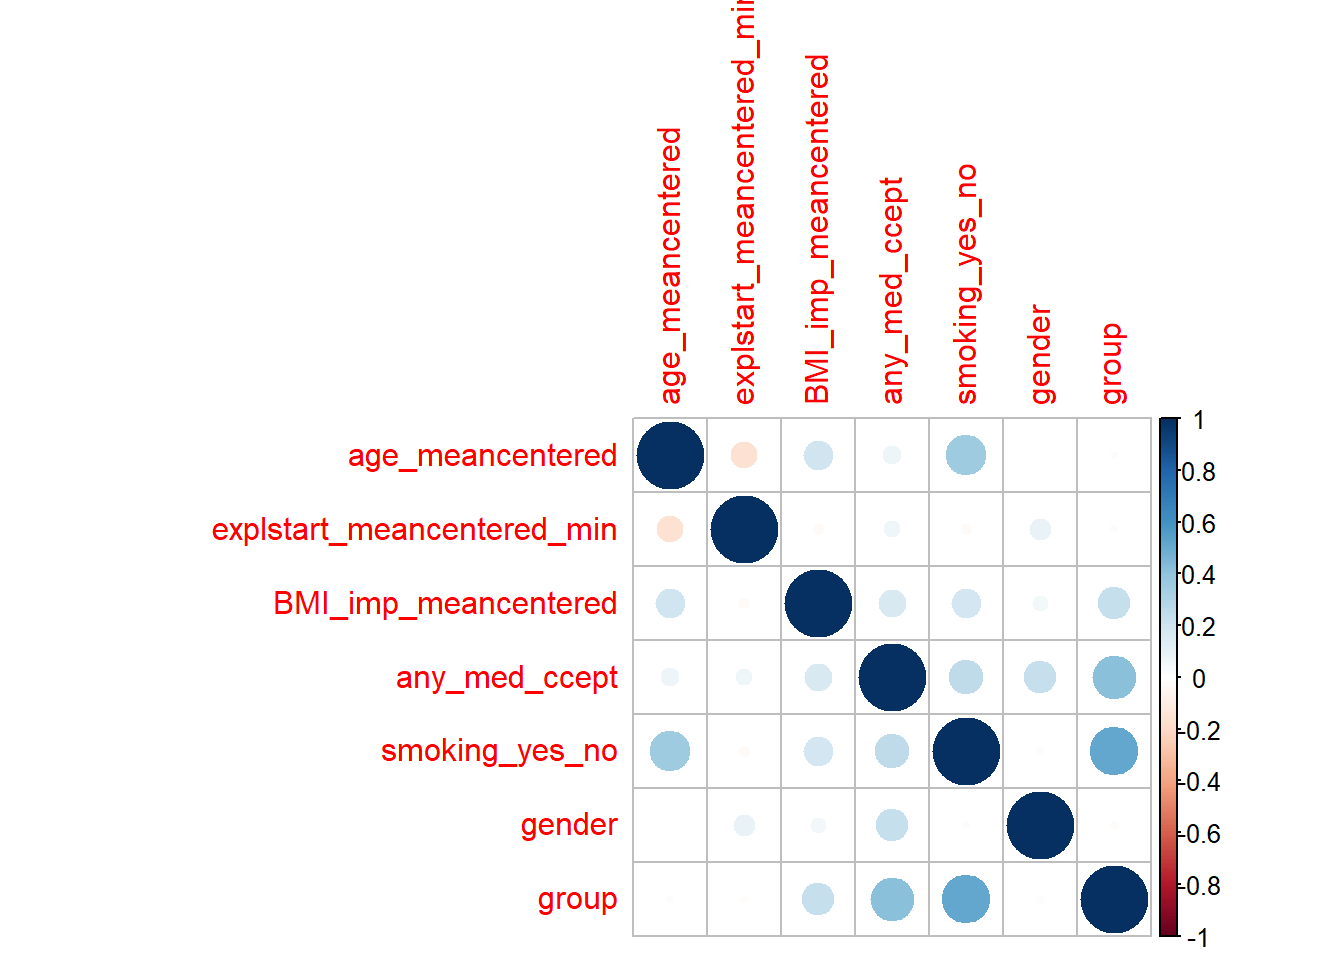
\includegraphics{01_Preprocessing_Modelling_files/figure-latex/preprocess-1.pdf}

\hypertarget{definitions}{%
\subsection{Definitions}\label{definitions}}

\textbf{IV of interest :}

\begin{itemize}
\tightlist
\item
  Gruppe (``group'')
\item
  sex (``gender'')
\item
  Zeitpunkt (``time'')
\item
  Gruppe x Zeitpunkt
\item
  Gruppe x sex
\end{itemize}

\textbf{IV of no interest :}

\begin{itemize}
\tightlist
\item
  Site (``centre'')
\item
  Age scaled (``age\_meancentered'')
\item
  ``explstart\_meancentered\_min''
\item
  ``BMI\_imp\_meancentered''
\item
  ``any\_med\_ccept''
\item
  ``smoking\_yes\_no''
\end{itemize}

\textbf{DV:}

\begin{itemize}
\tightlist
\item
  psychologischer Stress („stressed``)
\item
  Cortisol („CORT``)
\item
  Testosteron („TEST'')
\item
  Oxytocin (OXT'')
\end{itemize}

\hypertarget{linear-model-with-mixed-effects}{%
\subsection{linear model with mixed
effects}\label{linear-model-with-mixed-effects}}

We adapted a boxed design by individual over time

full model:
DV\textasciitilde1+centre+age\_meancentered+explstart\_meancentered\_min+BMI\_imp\_meancentered+any\_med\_ccept+smoking\_yes\_no+gender+group+time+gender\emph{group+time}group+gender\emph{time}group+(1\textbar twuid)

\begin{Shaded}
\begin{Highlighting}[]
\NormalTok{resall }\OtherTok{=} \FunctionTok{list}\NormalTok{()}

\ControlFlowTok{for}\NormalTok{ (depvar }\ControlFlowTok{in} \FunctionTok{names}\NormalTok{(AV))\{}
\NormalTok{  long }\OtherTok{=}\NormalTok{ df[,}\FunctionTok{c}\NormalTok{(}\StringTok{"twuid"}\NormalTok{, AV[[depvar]],UV)] }\SpecialCharTok{\%\textgreater{}\%} 
    \FunctionTok{gather}\NormalTok{(}\AttributeTok{key =} \StringTok{"value"}\NormalTok{, }\AttributeTok{value =} \StringTok{"DV"}\NormalTok{, AV[[depvar]])}
\NormalTok{  long}\SpecialCharTok{$}\NormalTok{time }\OtherTok{=} \FunctionTok{as.numeric}\NormalTok{(}\FunctionTok{gsub}\NormalTok{(}\StringTok{"[A{-}Z a{-}z\_]*"}\NormalTok{, }\StringTok{""}\NormalTok{, long}\SpecialCharTok{$}\NormalTok{value))}
\NormalTok{  long}\SpecialCharTok{$}\NormalTok{twuid }\OtherTok{=} \FunctionTok{as.factor}\NormalTok{(long}\SpecialCharTok{$}\NormalTok{twuid)}
\NormalTok{  model.lme }\OtherTok{=}\NormalTok{ lme4}\SpecialCharTok{::}\FunctionTok{lmer}\NormalTok{(model, }\AttributeTok{data=}\NormalTok{long)}
\NormalTok{  model.lme0 }\OtherTok{=}\NormalTok{ lme4}\SpecialCharTok{::}\FunctionTok{lmer}\NormalTok{(DV}\SpecialCharTok{\textasciitilde{}}\DecValTok{1}\SpecialCharTok{+}\NormalTok{(}\DecValTok{1}\SpecialCharTok{|}\NormalTok{twuid), }\AttributeTok{data=}\NormalTok{long)}
\NormalTok{  anovah0 }\OtherTok{=} \FunctionTok{anova}\NormalTok{(model.lme0, model.lme)}
\NormalTok{  model\_p\_val }\OtherTok{=}\NormalTok{ anovah0}\SpecialCharTok{$}\StringTok{\textasciigrave{}}\AttributeTok{Pr(\textgreater{}Chisq)}\StringTok{\textasciigrave{}}\NormalTok{[}\DecValTok{2}\NormalTok{]}
\NormalTok{  Res }\OtherTok{=} \FunctionTok{summary}\NormalTok{(model.lme)}
\NormalTok{  resall[[depvar]] }\OtherTok{=}\NormalTok{ model.lme}
\NormalTok{  res.coeff }\OtherTok{=} \FunctionTok{as.data.frame}\NormalTok{(Res}\SpecialCharTok{$}\NormalTok{coefficients)}
\NormalTok{  res.coeff}\SpecialCharTok{$}\NormalTok{pvalue }\OtherTok{=} \FunctionTok{pt}\NormalTok{(}\FunctionTok{abs}\NormalTok{(res.coeff}\SpecialCharTok{$}\StringTok{"t value"}\NormalTok{), }\DecValTok{1000000}\NormalTok{, }\AttributeTok{lower.tail =}\NormalTok{ F) }\SpecialCharTok{*} \DecValTok{2}
\NormalTok{  resall[[}\FunctionTok{paste0}\NormalTok{(depvar,}\StringTok{"\_coeff"}\NormalTok{)]]}\OtherTok{=}\NormalTok{res.coeff}
\NormalTok{  resall[[}\FunctionTok{paste0}\NormalTok{(depvar,}\StringTok{"\_modsig"}\NormalTok{)]]}\OtherTok{=}\NormalTok{model\_p\_val}
\NormalTok{\}}
\end{Highlighting}
\end{Shaded}

\begin{verbatim}
## refitting model(s) with ML (instead of REML)
## refitting model(s) with ML (instead of REML)
## refitting model(s) with ML (instead of REML)
## refitting model(s) with ML (instead of REML)
\end{verbatim}

\hypertarget{results}{%
\section{Results}\label{results}}

\hypertarget{stressed}{%
\subsection{stressed}\label{stressed}}

overall model p-value (h0 model:
stressed\textasciitilde1+(1\textbar twuid)): 8.86e-64

\begin{Shaded}
\begin{Highlighting}[]
\NormalTok{tableplot }\OtherTok{=} \ControlFlowTok{function}\NormalTok{ (x)\{}
\NormalTok{  x }\SpecialCharTok{\%\textgreater{}\%}\NormalTok{ dplyr}\SpecialCharTok{::}\FunctionTok{mutate\_if}\NormalTok{(is.numeric, }\ControlFlowTok{function}\NormalTok{(x)\{}\FunctionTok{as.character}\NormalTok{(}\FunctionTok{signif}\NormalTok{(x, }\DecValTok{3}\NormalTok{))\}) }\SpecialCharTok{\%\textgreater{}\%} \FunctionTok{kbl}\NormalTok{() }\SpecialCharTok{\%\textgreater{}\%} \FunctionTok{kable\_classic}\NormalTok{()}
\NormalTok{  \}}

\NormalTok{resall[[}\StringTok{"AV\_stressed\_coeff"}\NormalTok{]] }\SpecialCharTok{\%\textgreater{}\%} \FunctionTok{tableplot}\NormalTok{()}
\end{Highlighting}
\end{Shaded}

\begin{table}
\centering
\begin{tabular}[t]{l|l|l|l|l}
\hline
  & Estimate & Std. Error & t value & pvalue\\
\hline
(Intercept) & 3.04 & 0.233 & 13.1 & 6.38e-39\\
\hline
centreAAC & -0.463 & 0.381 & -1.21 & 0.225\\
\hline
centreBLB & -0.478 & 0.34 & -1.41 & 0.16\\
\hline
centreBCN & 0.144 & 0.269 & 0.536 & 0.592\\
\hline
centreSZG & 0.00724 & 0.295 & 0.0245 & 0.98\\
\hline
age\_meancentered & -0.0109 & 0.0562 & -0.193 & 0.847\\
\hline
explstart\_meancentered\_min & -0.00108 & 0.00176 & -0.611 & 0.541\\
\hline
BMI\_imp\_meancentered & 0.0268 & 0.0198 & 1.35 & 0.176\\
\hline
any\_med\_cceptmed & 0.18 & 0.252 & 0.713 & 0.476\\
\hline
smoking\_yes\_nosmk & 0.302 & 0.262 & 1.15 & 0.25\\
\hline
genderfemale & -0.654 & 0.345 & -1.9 & 0.0578\\
\hline
groupCD & 0.255 & 0.358 & 0.713 & 0.476\\
\hline
time & -0.35 & 0.0282 & -12.4 & 2.05e-35\\
\hline
genderfemale:groupCD & -0.142 & 0.512 & -0.278 & 0.781\\
\hline
groupCD:time & 0.0184 & 0.0424 & 0.433 & 0.665\\
\hline
genderfemale:time & 0.0615 & 0.0476 & 1.29 & 0.196\\
\hline
genderfemale:groupCD:time & 0.0362 & 0.0706 & 0.513 & 0.608\\
\hline
\end{tabular}
\end{table}

\hypertarget{cort}{%
\subsection{CORT}\label{cort}}

overall model p-value (h0 model:
stressed\textasciitilde1+(1\textbar twuid)): 2.17e-50

\begin{Shaded}
\begin{Highlighting}[]
\NormalTok{resall[[}\StringTok{"AV\_CORT\_coeff"}\NormalTok{]] }\SpecialCharTok{\%\textgreater{}\%} \FunctionTok{tableplot}\NormalTok{()}
\end{Highlighting}
\end{Shaded}

\begin{table}
\centering
\begin{tabular}[t]{l|l|l|l|l}
\hline
  & Estimate & Std. Error & t value & pvalue\\
\hline
(Intercept) & 1.65 & 0.0743 & 22.2 & 2.15e-109\\
\hline
centreAAC & 0.0782 & 0.137 & 0.569 & 0.57\\
\hline
centreBLB & -0.109 & 0.123 & -0.89 & 0.373\\
\hline
centreBCN & -0.0967 & 0.0971 & -0.996 & 0.319\\
\hline
centreSZG & -0.0777 & 0.107 & -0.729 & 0.466\\
\hline
age\_meancentered & 0.0938 & 0.0203 & 4.63 & 3.73e-06\\
\hline
explstart\_meancentered\_min & -0.00222 & 0.000636 & -3.5 & 0.000466\\
\hline
BMI\_imp\_meancentered & 0.00789 & 0.00712 & 1.11 & 0.268\\
\hline
any\_med\_cceptmed & -0.0654 & 0.091 & -0.718 & 0.473\\
\hline
smoking\_yes\_nosmk & -0.128 & 0.0945 & -1.36 & 0.175\\
\hline
genderfemale & -0.158 & 0.104 & -1.52 & 0.13\\
\hline
groupCD & -0.544 & 0.115 & -4.75 & 2.08e-06\\
\hline
time & -0.0107 & 8e-04 & -13.4 & 1.06e-40\\
\hline
genderfemale:groupCD & 0.139 & 0.155 & 0.9 & 0.368\\
\hline
groupCD:time & 0.00774 & 0.00119 & 6.52 & 7.05e-11\\
\hline
genderfemale:time & 0.00475 & 0.0013 & 3.66 & 0.00025\\
\hline
genderfemale:groupCD:time & -0.00495 & 0.00192 & -2.57 & 0.0101\\
\hline
\end{tabular}
\end{table}

\hypertarget{test}{%
\subsection{TEST}\label{test}}

overall model p-value (h0 model:
stressed\textasciitilde1+(1\textbar twuid)): 7.14e-28

\begin{Shaded}
\begin{Highlighting}[]
\NormalTok{resall[[}\StringTok{"AV\_TEST\_coeff"}\NormalTok{]] }\SpecialCharTok{\%\textgreater{}\%} \FunctionTok{tableplot}\NormalTok{()}
\end{Highlighting}
\end{Shaded}

\begin{table}
\centering
\begin{tabular}[t]{l|l|l|l|l}
\hline
  & Estimate & Std. Error & t value & pvalue\\
\hline
(Intercept) & 3.71 & 0.0631 & 58.8 & 0\\
\hline
centreAAC & 0.341 & 0.118 & 2.9 & 0.00378\\
\hline
centreBLB & -0.0391 & 0.105 & -0.372 & 0.71\\
\hline
centreBCN & 0.044 & 0.083 & 0.531 & 0.596\\
\hline
centreSZG & 0.209 & 0.0911 & 2.29 & 0.0218\\
\hline
age\_meancentered & 0.0733 & 0.0174 & 4.23 & 2.38e-05\\
\hline
explstart\_meancentered\_min & -0.00222 & 0.000543 & -4.08 & 4.43e-05\\
\hline
BMI\_imp\_meancentered & 0.0196 & 0.00611 & 3.21 & 0.00134\\
\hline
any\_med\_cceptmed & -0.121 & 0.078 & -1.56 & 0.119\\
\hline
smoking\_yes\_nosmk & 0.0865 & 0.0809 & 1.07 & 0.285\\
\hline
genderfemale & 0.231 & 0.089 & 2.6 & 0.00945\\
\hline
groupCD & -0.217 & 0.0975 & -2.22 & 0.0262\\
\hline
time & -0.00406 & 0.000563 & -7.2 & 5.94e-13\\
\hline
genderfemale:groupCD & 0.217 & 0.132 & 1.64 & 0.1\\
\hline
groupCD:time & 0.00376 & 0.000848 & 4.44 & 9.15e-06\\
\hline
genderfemale:time & 0.00402 & 0.000952 & 4.23 & 2.37e-05\\
\hline
genderfemale:groupCD:time & -0.00474 & 0.00141 & -3.36 & 0.000787\\
\hline
\end{tabular}
\end{table}

\hypertarget{oxt}{%
\subsection{OXT}\label{oxt}}

overall model p-value (h0 model:
stressed\textasciitilde1+(1\textbar twuid)): 0.394

\begin{Shaded}
\begin{Highlighting}[]
\NormalTok{resall[[}\StringTok{"AV\_OXT\_coeff"}\NormalTok{]] }\SpecialCharTok{\%\textgreater{}\%} \FunctionTok{tableplot}\NormalTok{()}
\end{Highlighting}
\end{Shaded}

\begin{table}
\centering
\begin{tabular}[t]{l|l|l|l|l}
\hline
  & Estimate & Std. Error & t value & pvalue\\
\hline
(Intercept) & 0.35 & 0.0748 & 4.68 & 2.81e-06\\
\hline
centreAAC & -0.0125 & 0.131 & -0.0956 & 0.924\\
\hline
centreBLB & -0.0699 & 0.112 & -0.625 & 0.532\\
\hline
centreBCN & -0.126 & 0.119 & -1.06 & 0.288\\
\hline
centreSZG & -0.0936 & 0.199 & -0.47 & 0.638\\
\hline
age\_meancentered & 0.0319 & 0.02 & 1.6 & 0.111\\
\hline
explstart\_meancentered\_min & 4.66e-05 & 0.000862 & 0.0541 & 0.957\\
\hline
BMI\_imp\_meancentered & -0.00883 & 0.00629 & -1.4 & 0.161\\
\hline
any\_med\_cceptmed & -0.0217 & 0.0865 & -0.251 & 0.802\\
\hline
smoking\_yes\_nosmk & 0.0821 & 0.0919 & 0.893 & 0.372\\
\hline
genderfemale & -0.0976 & 0.101 & -0.97 & 0.332\\
\hline
groupCD & -0.0627 & 0.119 & -0.527 & 0.598\\
\hline
time & -0.00144 & 0.00194 & -0.744 & 0.457\\
\hline
genderfemale:groupCD & -0.113 & 0.154 & -0.738 & 0.461\\
\hline
groupCD:time & 0.00993 & 0.00764 & 1.3 & 0.194\\
\hline
genderfemale:time & -0.00125 & 0.00279 & -0.447 & 0.655\\
\hline
genderfemale:groupCD:time & 0.00188 & 0.0115 & 0.163 & 0.87\\
\hline
\end{tabular}
\end{table}

\end{document}
